\subsection{Sparse-overlapping-sets (SOS) LASSO}
\subsubsection{Concepts and assumptions}
The multivariate methods we have considered so far lie at two poles with regard to their assumptions. The searchlight method assumes both localization of signal within individuals, and consistency of localization across individuals. Regularized regression discards both assumptions, allowing for the possibility that representations of interest are arbitrarily situated within individuals, in completely different ways across individuals. From the PDP view of representation, the former assumptions seem too restrictive, while the latter assumptions seem too loose. If we believe that all human beings share the same gross neuroanatomical structure, then it seems reasonable to suppose {\em some degree} of localization within individuals and some degree of consistency in location across individuals. Within individuals we might assume that, if a given unit is important for representation, there is a good chance that some other units in the general vicinity are also important. Such an assumption could be adopted without further requiring that {\em all} neighboring units are important (univariate assumption X), or that neighboring units contain sufficient information for the representation (searchlight assumption X). Likewise we might assume that, if a set of voxels contribute to a representation in individual A, then, in individual B, signal-carrying voxels are likely to be found in the same general vicinity. Such an assumption could be adopted without requiring that the location of the interesting information is very precisely aligned, or that the location contains useful information in the great majority of individuals (univariate and searchlight assumptions X).

The final method we consider is a variant of LASSO that assumes a loose degree of localization within individuals and a loose degree of consistency in location across individuals. The general approach is based on {\em multi-task learning} whose conceptual basis is intuitive: it assumes that, if two learning tasks are related in some way, then their solutions will be related. In this case, each ``task'' is to find the representation of interest in a single individual. In contrast to LASSO, we assume that the solutions across individuals are related: finding useful information in one individual gives us clues about where to look in another. The loose assumptions about localization within and across individuals can be built into a single optimization function that considers all subjects at once.

The method works as follows. The voxels for each individual are first projected into a common anatomical reference space (without blurring). The space is divided into a 3-dimensional grid and, for each gridpoint, all voxels within radius $r$ are grouped together in a $set$. Each set thus contains a group of anatomically proximal voxels; each voxel belongs to multiple sets; and the sets overlap in the voxels they contain. The sets are thus analogous to searchlights. Rather than training separate classifiers for each set and subject, however, a regularized logistic classifier is trained on all the data together. In this case, the regularization penalty contains two terms. One term scales linearly with the number of sets included in the solution; the other is the standard LASSO penalty across all units:

{\em equation here?}

Overall, the joint optimization prefers solutions that (a) fit the training data by (b) finding units that belong to a small number of sets and (c) include a relatively small proportion of the units overall. The optimization places a separate weight on each unit for each individual, and in this sense allows for complete variability across individuals in how information is encoded. It also ``sees'' all units in the brain at once, and so can be sensitive to information distributed over several different anatomical regions. But, it prefers solutions where the informative features within an individual are situated in the same small number of sets across individuals, thus implementing the assumptions of loose localization within loose consistency of location across individuals. A mathematical analysis of \soslasso and some applications of its use were recently described by \cite{RaoNIPS} for linear regression and by \cite{RaoML} for logistic regression. 

Relative to other methods, \soslasso thus adopts the following assumptions about representation
\begin{enumerate}
\item Localization within individuals: Loose localization is assumed. Representational elements are assumed to reside in a number of anatomical clusters. However, units within a cluster are not assumed to {\em all} contribute to the representation; and each cluster is not assumed to individual contain sufficient information about the representation.

\item Consistency of coding within individual representations: No consistency in how information is encoded within a representation is assumed.

\item Localization across individuals: Representations are assumed to be localized in loosely similar ways across individuals. The informative units are assumed to reside in roughly similar locations, but these need not be identical, and a given location need not contain useful information for most individuals.

\item Consistency of coding across individuals: No consistency of coding across individuals is assumed.

\item Independence of representational units: The approach does not assume that units code information independently.

\item Sparsity: The representation is assumed to be sparse.

\item Redundancy: The representation is assumed to have low redundancy.
\end{enumerate}

With these assumptions, how does the approach fare in analysis of model data?

\subsubsection{Implementation} 
The \soslasso analysis was implemented using custom code built on top of the MALSAR package\cite{malsar} for \matlab. The data were divided into overlapping sets based on ``anatomical'' proximity. Each set included 5 units, and the sets overlapped with each other by 2 units. The set size was kept smaller than the smallest expected cluster of informtive units in the localized data, but otherwise arbitrary. \soslasso has two free parameters, one controlling sparsity at the set level and one controlling overall sparsity. As in the previous analysis, these parameter values  were selected through an internal 5-fold cross-validation process, then a final model was trained with the best parameters and tested on a sixth hold-out set. Note that \soslasso is trained on all model subjects simultaneously, but produces a unique solution for each subject. Thus the results were analyzed in the same way as the LASSO and ridge regression results.

\subsubsection{Results}
\textbf{---Figure 9 about here---}
\begin{figure}
\centering
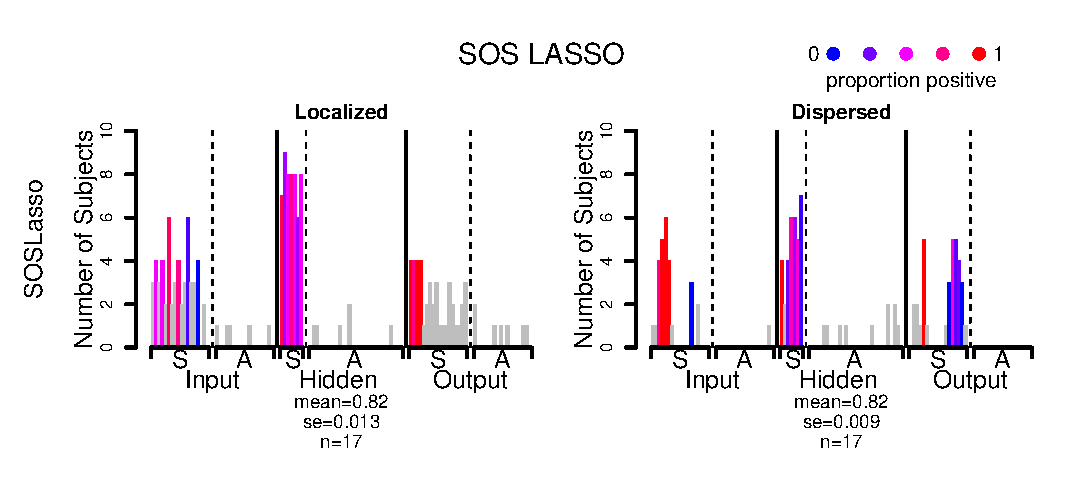
\includegraphics[width=0.75\textwidth]{figures/soslasso_only.eps}
\caption{\label{fig.sos} The results from the three regularized regression analyses. Because the model weights themselves are biased estimates and on an arbitrary scale, the height of each bar corresponds to the number of number of times each unit was selected over subjects. Colored bars were selected more times than would be expected given the overall rate of unit selection. The blueness or redness of the bar conveys the proportion of the time each unit was assigned a positive weight over subjects. Positive weights mean that activation at that unit will push the model towards labeling the current item as belonging to domain A.}
\end{figure}

The first point of note is that the \soslasso classifier showed a mean cross-validation accuracy across subjects of 0.82 in both the localized and anatomically dispersed model variants--much higher than searchlight, LASSO, and ridge regression, all of which showed accuracies between 0.6-0.65. This stark difference suggests that \soslasso is able to exploit cross-subject consistency in the location of useful units to better find the informative signal in individual models.

Figure \ref{fig.sos} shows, for each unit, how frequently it was identified as important across model individuals. As with LASSO, the base-rate of unit selection was used to conduct a binomial test across model individuals, to indicate which units were selected more often than expected by chance. The method clearly excels at identifying the SH units. When these are localized, all units are reliably identified, but even when they are anatomically dispersed, the method reliably finds 6 of the 7 units. Arbitrary units are almost never flagged as important for representation. Compared to LASSO, the method also does a slightly better job identifying the systematic I/O units, reliably identifying 11 of the 36 units (31\%) in both cases.

The rightmost panel of Figure \ref{fig.precision} shows the mean precision and hit rate across individuals in the anatomically localized and dispersed models. Considering all units, \soslasso maintains the same precision as LASSO, but with a substantially better hit rate. With localized representations, this improvement was observed for both hidden and I/O units. When hidden representations were anatomically dispersed, the precision declined slightly but the hit rate still improved markedly. In the dispersed case the precision declines when the method sometimes selects arbitrary units belonging to sets containing signal-carrying units. An arbitrary unit contained in a selected set and happening to spuriously covary with the class label may itself be selected. Despite such inclusions, however, the overall gain in hit rate with minimal loss of precision, together with the greatly improved classifier cross-validation accuracy, suggest that \soslasso is doing a substantially better job of finding useful representational structure.

The advantages of \soslasso are clear when representations are anatomically localized, but what accounts for the improved hit rate when they are dispersed? The first observation is that, though signal-carrying voxels do not line up across subjects, there exist some unit sets that happen to contain many signal-carrying voxels across subjects, while others contain mostly arbitrary voxels.\soslasso places zero weights on sets with many arbitrary voxels but selects those with signal-carriers, since these help reduce classification error. If this were the only reason, however, then the searchlight method should have also succeeded. The second observation is that all of the selected voxels across sets contribute to a single classifier, just as in LASSO and ridge regression. Thus \soslasso can perform well even when the useful information is distributed over multiple sets. In general \soslasso builds the best sparse whole-brain classifier possible while keeping solutions for different subjects as similar as possible, where similarity is defined by membership in the same set.

It is worth noting here that the \soslasso is a generalized optimzation within which LASSO itself is a special case. When the parameter controlling the weight on the group sparsity penalty is set to zero, the regularizer reduces to the standard LASSO penalty. This means that the parameterization of \soslasso itself indicates the extent to which there exists useful cross-subject consistency in signal location. If no such consistency exists, the classifier cross-validation accuracy will not exceed that of LASSO alone, and the best estimate for the group-sparsity parameter will be near zero. For real data, this suggests a way of testing whether there exists cross-subject consistency in information localization. The \soslasso classifier will only perform better than the LASSO classifier if such consistency exists.

Finally, with regard to laying bare the representational code, \soslasso performs similarly to LASSO: Where units are reliably discovered, the nature of the code is clear from the weight values (colored bars in Figure \ref{fig.sos}), though these patterns are somewhat noisy when the units are only discovered in a small number of model individuals.

In sum, \soslasso shows the following answers to the core questions: 

\begin{enumerate}
\item {\bf Does the method reliably identify the systematic I/O units?} It does so better than LASSO, but not as well as searchlight or univariate analysis. The method assumes an overall sparse representation, and so will find a small set of units that strongly encode the information of interest. Where signal is weakly coded across many redundant units, \soslasso will still tend to miss many units.
\item {\bf Does the method reliably identify the systematic hidden units?} Yes---of all methods, \soslasso has the highest hit rate and precision for the SH units, in both localized and dispersed cases.
\item {\bf Does the method indicate how the information of interest is coded across identified units?} Like LASSO, it does so quite well for identified units, though few I/O units are identified and each SH unit is only identified in about half of the individuals.
\item {\bf Do method results depend on anatomical localization of signal-carrying units?} Somewhat: The method had slightly lower precision and hit rates among hidden units when these were anatomically dispersed, though the effects were much milder than those observed for searchlight.
\end{enumerate}